\documentclass[aps,letterpaper,11pt]{revtex4}

\usepackage{graphicx}
\usepackage{float}
\usepackage{verbatim}
\usepackage{amsmath}
\usepackage{amssymb}

\newcommand{\labno}{6}
\newcommand{\labtitle}{Comparing Tension and Acceleration of an Object Moving on an Incline with Friction}
\newcommand{\authorname}{Kevin Truong}
\newcommand{\professor}{Dr. Melanie Lutz}
\newcommand{\classno}{Physics 006}
\newcommand{\labpartners}{Sean Casey, Kevin Castillo, and Dulce Payan}
\newcommand{\submitdate}{March 28,2017}

\begin{document}

\begin{titlepage}
\begin{center}
\hspace{-136mm}\boxed{{\Large \textsc{Lab No. \labno}}}\\\vspace{30mm}
{\Large \textsc{\labtitle} \\ \vspace{4pt}}
\rule[13pt]{\textwidth}{1pt}\\ \vspace{150pt}
{\large By: \authorname \\ \vspace{10pt}}
Lab Partners: \labpartners \\
Instructor: \professor \vspace{10pt} \\
Solano Community College\\ \classno \\ \vspace{10pt}
\submitdate
\end{center}
\end{titlepage}

\section{Abstract}

An "Atwood's Machine" was used to compare tension in a string between a cart and a hanging mass when the cart is at rest and when the cart is accelerating towards the pulley. When comparing these two tensions the tension of the system at rest was greater than the tension of the system that was accelerating due to the hanging mass. The tension as the system accelerated was less because some of the force within the tension went to the acceleration of the masses. The calculated theoretical tension as the system was at rest was 1.96N. The calculated theoretical tension as the system was accelerating was 1.52N and the calculated theoretical acceleration was 2.20$\frac{m}{s^2}$. After the experiment concluded, the experimental tension as the system was at rest was 1.972N, the experimental tension as the system was accelerating was 1.525N, and the experimental acceleration collected from the motion detector was 2.047$\frac{m}{s^2}$. using the percent error equation, the percent error between the theoretical tension and the experimental tension as the system was at rest was .612\%. The percent error between the theoretical tension and the experimental tension as the system was accelerating was .329\%. The percent error between the theoretical acceleration and the experimental acceleration was 6.91\%. These percent errors might be due to inaccuracies in the equipment used. When comparing the experimental tension value as the system was at rest (1.972N) to the experimental tension value as the system was accelerating (1.525N), it is possible to see that the tension while the system was at rest is greater than the tension while the system is accelerating towards the pulley.



\section{Introduction}

Analyzing Newton's second law, there is a direct relationship between force and acceleration; $F=ma.$ The relationship between force and acceleration in Newton's second law is important because knowing the acceleration or force of an object could help solve for other information such as mass, velocity, distance, etc. More formally, Newton's second law is defined as the net force acting on the body equalling to the objects mass times its acceleration. Force is a vector quantity, therefore force can be broken up into components; $\sum_{}^{}\vec{F} = \sum_{}^{}\vec{F_x} + \sum_{}^{}\vec{F_y}$. The individual components can be analyzed and valuable information can be obtain by looking at the individual components of force. 

A body is static when it is at rest or has constant velocity, this means that the acceleration of the object is zero. In the case of a static body, the net force on the body would equal zero. When analyzing an "Atwood's Machine" it's important to analyze all of the components of force to obtain valuable information, even when the object being analyzed is static.

Percent error is imporant in understanding the accuracy of the data collected to the theoretically calculated data. To understand the possible flaws that will skew the accuracy of the data. Percent error can be calculated using the equation:

$$ \% \hspace{1mm} error = |\frac{a_{experimental} - a_{theoretical}}{a_{theoretical}}|*100\%$$

\section{Experimental Details}

Equipments for this experiment includes a ramp, cart, 0.05kg mass, string, pulley, motion detector, and computer. The ramp was the medium for the cart to move on, the surface of the ramp had friction. The cart was pushed up and down the ramp, it is the object being analyzed throughout this experiment. The 0.05kg mass was attached to the cart using a string and was hung from a pulley, it accelerates with the cart. The String kept the cart and the hanging mass linked together. The pulley was used to keep a smooth movement between the cart and the hanging mass. The motion detector was used to calculate the acceleration, velocity, and position of the moving cart. The computer was used to process the collected data of the motion detector through the Logger Pro program. 

For part A of the experiment, we found the coefficient of friction of the track by simply pushing the cart on the ramp when it was straight horizontal with the table. We did this by using the motion detector analyzing, on the computer, how the cart slowed down due to the friction of the ramp. The following is the diagram for part A, where the cart was pushed and analyzed using the motion detector; we did this three times and found the average coefficient of friction to have a more accurate calculation of the coefficient of friction.

\begin{center}
\underline{Diagram 1}\\
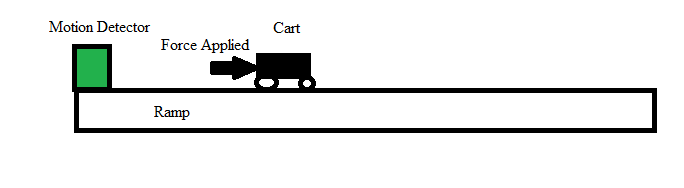
\includegraphics[width=4in]{SetupPartA.png}\\
\textit{Diagram 1: Setup for the part A of the experiment}
\end{center}

Equipment for this experiment includes a force sensor and force sensor hook, motion detector, cart, "frictionless" ramp, 1.0kg and 0.2kg masses, string, and a computer with Logger Pro Program. The force sensor and force sensor hook were used to collect the tension force between the cart and the hanging mass. The motion detector was used to collect the movement of the cart as it accelerated due to the weight of the hanging mass. The cart was used as mass one and stayed horizontal on the ramp. The "frictionless ramp" was used to simulate a frictionless system for the cart's movement. The 1.0kg mass was used to calibrate the force sensor while the 0.2 kg mass was mass two that was hanging and pulling mass one to move horizontally across the ramp. The string will be used to attach cart to the hanging mass. The computer was used in tandem with the Logger Pro Program to organize the data collected by the force sensor and motion detector. 

When calibrating the force sensor, it is possible to do so by using the 1kg mass as the hanging mass while the cart is stopped at the end stop of the ramp closest to the pulley. This will be set to 9.8N of force. 

The string that is connecting the cart to the hanging mass must be horizontal and flush with the top of the pulley.

The experiment will compare the tension of the string between the cart and the 0.2kg mass when the cart is at rest to the tension of the string between the cart and the 0.2kg mass  
when the cart is accelerating towards the string due to the acceleration of the hanging mass. 

\newpage

\begin{center}
\underline{Diagram 1}\\
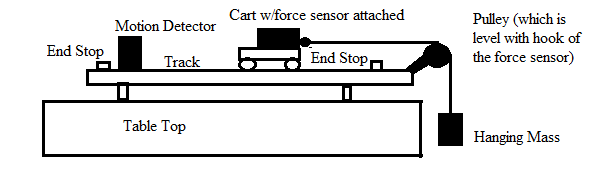
\includegraphics[width=6in]{Setup.png}\\
\textit{Diagram 1: Setup for experiment, to compare the different tensions of the string.}\\
\end{center}

It's necessary to find the mass of the cart to calculate the theoretical tensions and acceleration, this can be done by using a scale. The mass of the cart that was used for the experiment had a mass of 0.6915kg.

\section{Results and Analysis}

\subsection{Cart at Rest}

When the cart is at rest, it is static therefore it has an acceleration of zero. This was accomplished by setting the cart at the end stop, so the hanging mass wouldn't be able to pull the cart farther towards the pulley. When calculating the tension it is necessary to analyze the free body diagram of the system, let the tension of the string at rest be represented by $T_0$. In this case, it's possible to find an equation for $T_0$ by analyzing the free body diagram of mass 2 (the hanging mass).

\begin{center}
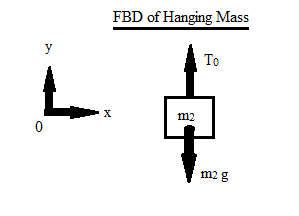
\includegraphics[width=4in]{FBDM2REST.png}\\
\end{center}

Looking at the summation of forces in the y-direction:

$$ \sum_{}^{} F_y = 0 $$

$$ T_0 - m_2g = 0$$

$$ \therefore T_0 = m_2g$$

The theoretical value of $T_0$ was then calculated with the known values of $m_2$ which was 0.2kg and gravity.

$$ T_0 = (0.2kg)(9.8\frac{m}{s})$$

$$ \boxed{T_0 = 1.96N}$$

\subsection{Cart Accelerating} 

In this portion of the experiment the cart is accelerating towards the pulley due to the hanging mass. This was accomplished by setting the cart a distance away from the end stop closest to the pulley, and then releasing the hanging mass causing the hanging mass to accelerate toward the floor and causing the cart to accelerate toward the pulley. Let the tension of the string as the cart is accelerating towards the pulley be represented as T.

In this scenario, the T is less than $T_0$. T is less than $T_0$ because there is acceleration at this point. Prior, when the cart was at rest, $T_0$ had to be equal to the weight to have the right side of newton's second law to equal zero. In this scenario, there is a quantity on the right side of newton's second law, and the only force acting against tension is the weight of the hanging mass just like when the cart is at rest, so T must be less than $T_0$ because if they were equal than the there would be no acceleration. 

When the cart is accelerating some of the force from the tension of the string is translated to the acceleration therefore the tension when the cart is accelerating is less than the tension when the cart is at rest.

An equation can also be derived to obtain the theoretical tension, T, and the theoretical acceleration for this portion of th experiment. The free body diagram of the handing mass would be the same as in part a:

\begin{center}
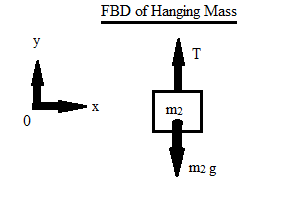
\includegraphics[width=4in]{FBDM2Accelerating.png}\\
\end{center} 

According to my axis, the acceleration($a_y$) would be in the negative direction.

$$ \sum_{}^{} F_y = m_2(-a_y) $$

$$ T - m_2g = -m_2a_y$$

$$ T = m_2(g-a_y)$$

Looking at the free body diagram on the cart:

\begin{center}
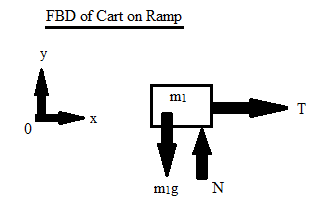
\includegraphics[width=4in]{FBD1Accelerating.png}\\
\end{center}

Here my acceleration would be in the positive direction:

$$ \sum_{}^{} F_x = ma_x$$

$$ T = m_1a_x$$

Since there is no acceleration in the y direction of this free body diagram, the right side of Newton's second law is zero.

$$ \sum_{}^{} F_y = 0$$

$$ N - m_1g = 0$$

$$ N = m_1g$$ 

According to my axis, $a_x = -a_y$; Let $a = a_x $ and $a = a_y$. Then we can equate the tension equations that was found, and solve for the acceleration:

$$ m_2g - m_2a = m_1a$$

Then we can solve for a:

$$ a = \frac{m_2g}{m_1 + m_2}$$

Now we can plug this into the equation that we found for tension:

$$ T = m_1(\frac{m_2g}{m_1 + m_2})$$

Since the equation for acceleration and tension were derived, it is possible to calculate the theoretical tension and acceleration. Plugging in the known values, the theoretical result:

$$ a = \frac{(0.2kg)(9.8\frac{m}{s^2})}{(0.6915kg) + (0.2kg)} = \boxed{2.20\frac{m}{s^2}}$$

$$ T = (0.6915kg)(2.20\frac{m}{s^2}) = \boxed{1.52N}$$

Comparing the theoretical equations for T and $T_0$, it is possible to see that $T_0 \geq T$. By comparing the equations: $m_2g \geq m_2g(\frac{m_1}{m_1 + m_2})$ because $\frac{m_1}{m_1+m_2}$ will be a fraction causing the value of T to be less than $T_0$. $T= T_0$ only when $m_2 = 0$. The numerical values show that $T_0 > T$.

\subsection{Measurements}

In this portion of the experiment, data was collected using the motion detector and force sensor. The cart was a distance away from the end stop closest to the pulley, and the hanging mass was released causing the cart to accelerate towards the pulley. The motion detector collected the acceleration values of the cart and the force sensor collected the force values on the cart. 

Figure 1 shows the acceleration vs. time graph that was collected and organized by the Logger Pro Program. 

\begin{center}
\underline{Figure 1}\\
\vspace{-30mm}
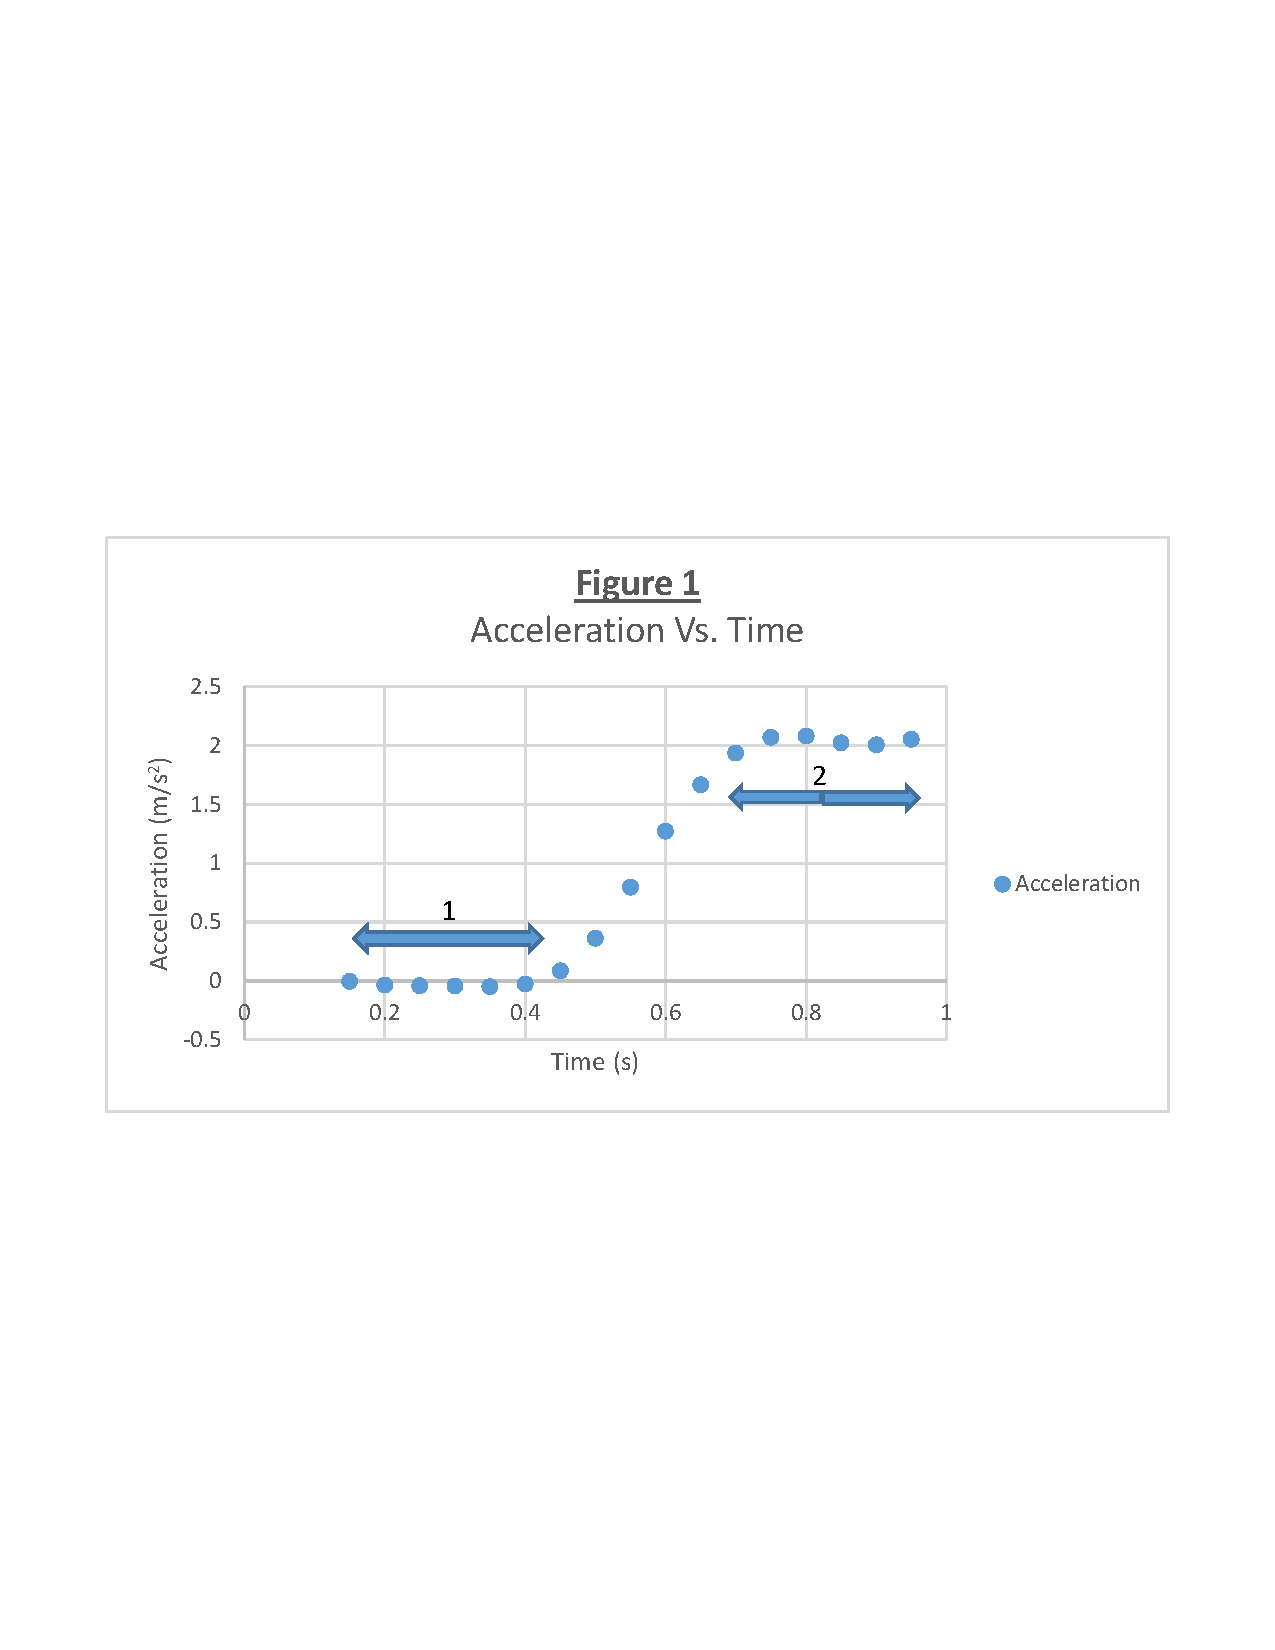
\includegraphics[width = 4in]{AccelerationVsTimeGraph.pdf}\\
\vspace{-40mm}
\textit{Figure 1: The time interval of 1 is the zero acceleration while the time interval of 2 is the constant acceleration.}
\end{center}

When analyzing the Acceleration Vs. Time graph on the Logger Pro Program, the mean value of the acceleration where it was approximately constant was 2.047$\frac{m}{s^2}$. This is the experimental value for the acceleration.

Calculating the percent error was possible using the equation:

$$ \% \hspace{1mm} error = |\frac{a_{experimental} - a_{theoretical}}{a_{theoretical}}|*100\%$$

$$ \% \hspace{1mm} error = |\frac{(2.047\frac{m}{s^2}) - (2.20\frac{m}{s^2})}{2.20\frac{m}{s^2}}|*100\% \boxed{\approx 6.91\%} $$

Figure 2 shows the Force vs. Time graph that was collected and organized by the Logger Pro Program.

\begin{center}
\underline{Figure 2}\\
\vspace{-30mm}
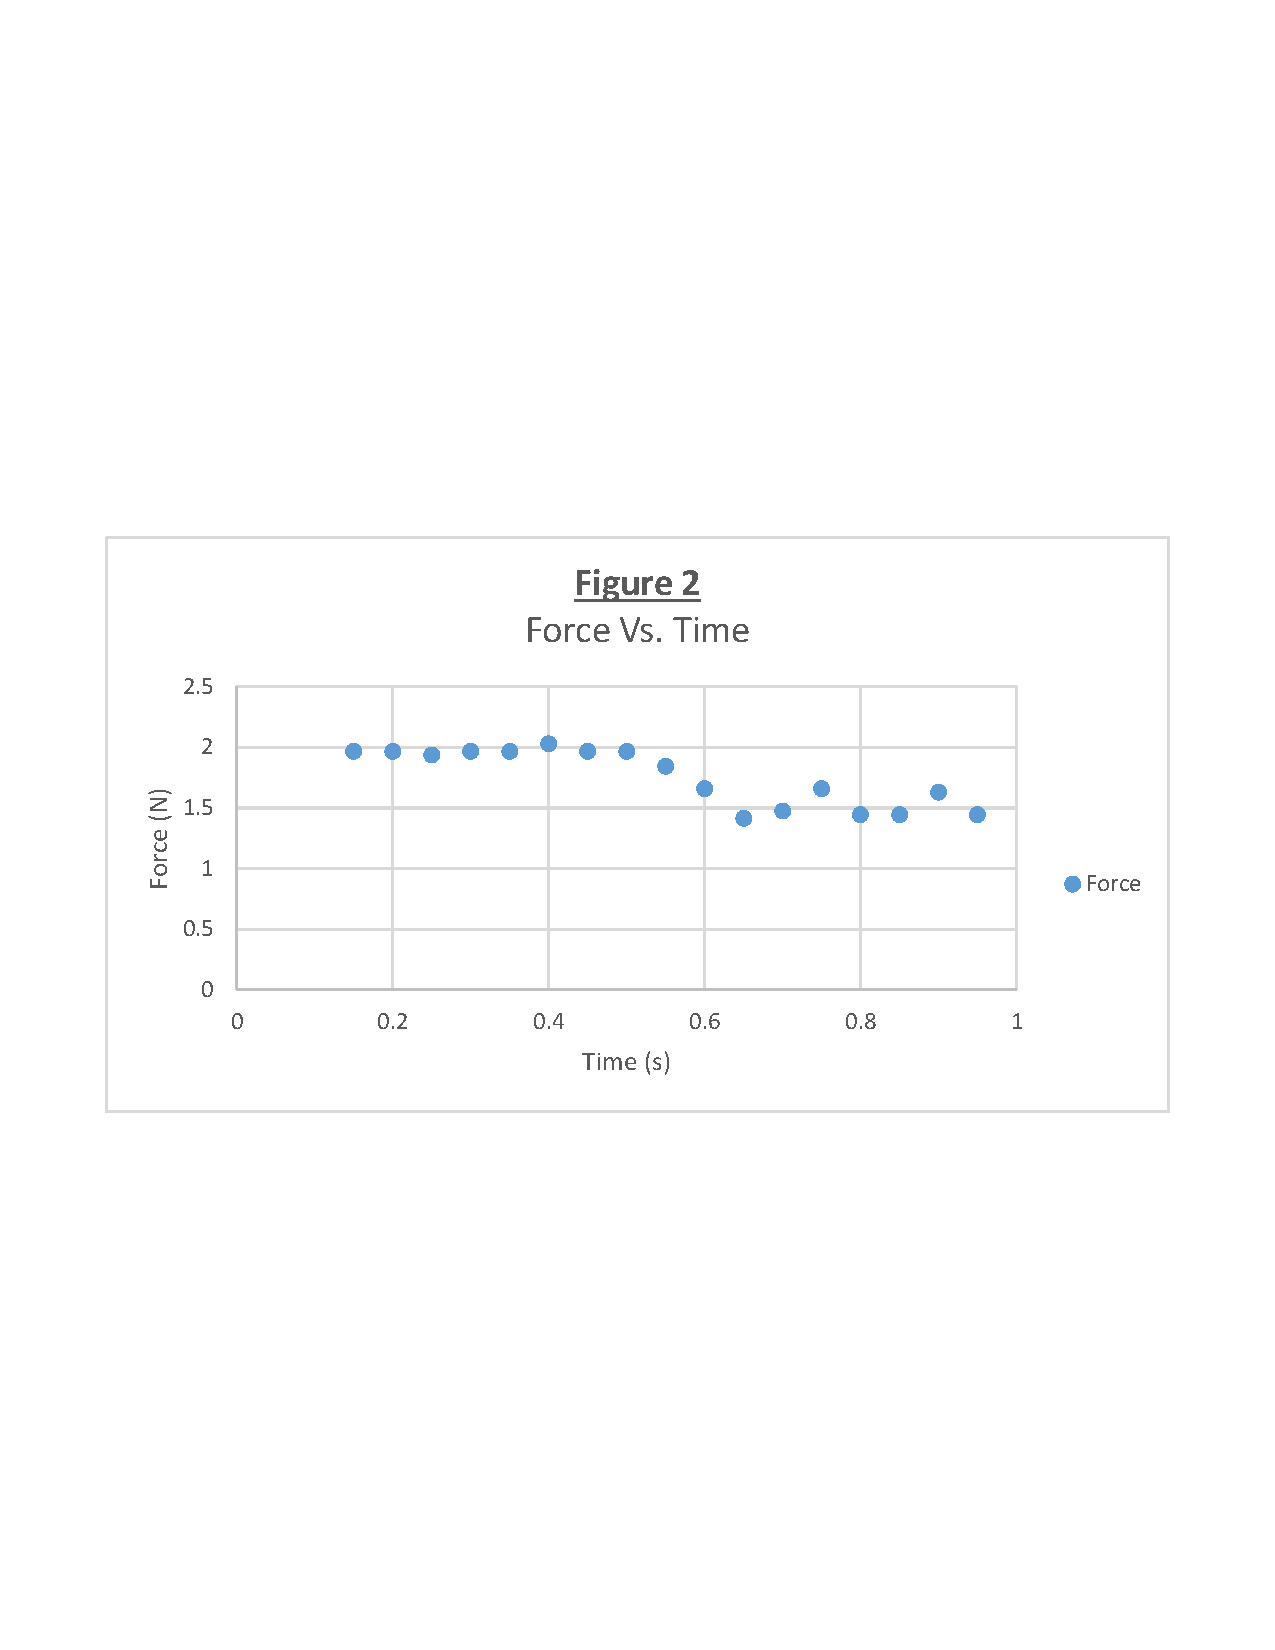
\includegraphics[width=4in]{ForceVsTimeGraph.pdf}\\
\vspace{-40mm}
\textit{Figure 2: Force vs. Time graph between the moving cart and hanging mass.}
\end{center}

Using the Logger Pro Program, the mean value of the force was obtained. The mean value of force was: 1.525N. Using the same \% error equation the \% error can be calculated comparing the theoretical value of force and the experimental value of force:

$$ \% \hspace{1mm} error = |\frac{(1.525N) - (1.52N)}{1.52N}|*100\% \boxed{\approx .329\%} $$

The force at the time interval of 1 in Figure 1, is when the acceleration is approximately zero. The mean value of force during this time interval was 1.972N. Again using the same \% percent error equation, the \% error can be calculated:

$$ \% \hspace{1mm} error = |\frac{(1.972N) - (1.96N)}{1.96N}|*100\% \boxed{\approx .612\%} $$.

The value of our percent errors show that the theoretical calculations were correct because the experimental values was very similar to the theoretical values.

\section{Discussion} 

The experiment showed that the tension($T_0$) of the string between the cart and the hanging mass when the cart is at rest was greater than the tension(T) of the string between the cart and the hanging mass when the cart is accelerating towards the pulley. 
T was less than $T_0$ because some of the force in the tension of the string went to the acceleration. The percent error of $T_0$, T, and a may have been due to inaccuracies in the eqiupment.  

\section{References}

\hspace{-6.5mm}
Force and Acceleration II Physics 06 Lab, Dr. Melanie Lutz\\



\end{document}
